\documentclass[11pt]{article}
\usepackage[T1]{fontenc}
\usepackage[utf8]{inputenc}
\usepackage{lmodern}
\usepackage{amsmath}
\usepackage{amssymb}
\usepackage{amsthm}
\usepackage{graphicx}
\usepackage[authoryear]{natbib}
\usepackage[colorlinks=true,linkcolor=blue,citecolor=blue,urlcolor=blue]{hyperref}
\newcommand{\R}{\mathbb{R}}
\newcommand{\norm}[1]{\left\lVert #1\right\rVert}

%% OverLyX ------------------------------------------------------------------
%% overlyx-settings: {"textclass":"article","cite_engine":"natbib","cite_engine_type":"authoryear","use_hyperref":"true","modules":["theorems-ams"]}
%% Packages and macros needed by the content (generated on every save; put your own preamble above this block).
\makeatletter
\providecommand{\LyX}{\texorpdfstring{%
  L\kern-.1667em\lower.25em\hbox{Y}\kern-.125emX\@}{LyX}}
%% Because html converters don't know tabularnewline
\providecommand{\tabularnewline}{\\}
\theoremstyle{plain}
\newtheorem{thm}{\protect\theoremname}
\theoremstyle{plain}
\newtheorem{lem}[thm]{\protect\lemmaname}
\makeatother
\providecommand{\theoremname}{Theorem}
\providecommand{\lemmaname}{Lemma}
%% end OverLyX --------------------------------------------------------------

\begin{document}
\title{A Short Paper Written in OverLyX}
\author{@@NAME@@}
\maketitle
\begin{abstract}
This is an example paper to start from. It has what most papers have --- sections, numbered equations with cross-references, a theorem with its proof, a figure, a table and citations from a Bib\TeX{} file --- and it is an ordinary \LaTeX{} file, so it compiles anywhere. Replace the text with your own, or keep it as a reference for how things look in OverLyX. The mathematics is a classic: gradient descent converges linearly on smooth, strongly convex functions.
\end{abstract}

\section{Introduction}\label{sec:intro}

We want to minimise a function $f\colon\R^{n}\to\R$. Gradient descent is the simplest method for this \citep{nocedal2006numerical}: starting from $x_{0}$, it steps against the gradient,
\begin{equation}
x_{k+1}=x_{k}-\eta\,\nabla f(x_{k}),\label{eq:gd}
\end{equation}
with a step size $\eta>0$. Momentum methods \citep{polyak1964some,nesterov1983method} add a multiple of the previous step and converge faster on ill-conditioned problems. \citet{boyd2004convex} give a thorough introduction to the convex case, on which we focus in Section~\ref{sec:theory}.

In OverLyX you edit this text as it will look in the PDF: a formula opens for editing when you click it, a citation shows its reference when you hover over it, and the outline on the right follows the sections.

\section{Convergence}\label{sec:theory}

We assume that $f$ is $L$-smooth and $\mu$-strongly convex, that is, for all $x,y\in\R^{n}$,
\begin{equation}
\frac{\mu}{2}\norm{y-x}^{2}\le f(y)-f(x)-\nabla f(x)^{\top}(y-x)\le\frac{L}{2}\norm{y-x}^{2},\label{eq:assumptions}
\end{equation}
and we write $f^{\ast}=\min_{x}f(x)$ and $\kappa=L/\mu$ for the condition number.
\begin{lem}
\label{lem:descent} With $\eta=1/L$, every step of \eqref{eq:gd} decreases $f$ by at least $\frac{1}{2L}\norm{\nabla f(x_{k})}^{2}$.
\end{lem}

\begin{proof}
Put $y=x_{k+1}$ and $x=x_{k}$ into the right inequality of \eqref{eq:assumptions}.
\end{proof}
\begin{thm}
\label{thm:linear} With $\eta=1/L$, gradient descent satisfies
\begin{equation}
f(x_{k})-f^{\ast}\le\left(1-\frac{1}{\kappa}\right)^{k}\left(f(x_{0})-f^{\ast}\right).\label{eq:rate}
\end{equation}
\end{thm}

\begin{proof}
Minimising both sides of the left inequality of \eqref{eq:assumptions} over $y$ gives $\norm{\nabla f(x)}^{2}\ge2\mu\left(f(x)-f^{\ast}\right)$. Together with Lemma~\ref{lem:descent}, $f(x_{k+1})-f^{\ast}\le\left(1-\mu/L\right)\left(f(x_{k})-f^{\ast}\right)$; the claim follows by induction.
\end{proof}

\section{Experiments}\label{sec:experiments}

Figure~\ref{fig:convergence} compares the error of the three methods on a quadratic with $\kappa=100$, and Table~\ref{tab:iterations} counts the iterations they need. The numbers are illustrative: replace them with your own results.

\begin{figure}
\centering
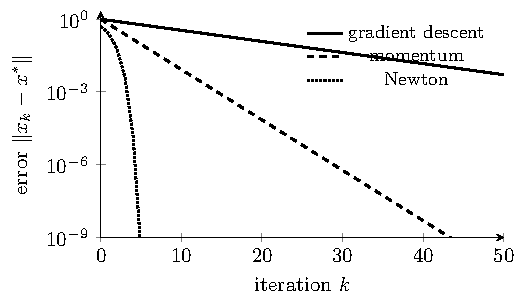
\includegraphics[width=0.75\textwidth]{figures/convergence} \caption{Error against iterations. Gradient descent converges linearly, as Theorem~\protect\ref{thm:linear} predicts; momentum improves the rate from $1-1/\kappa$ to about $1-1/\sqrt{\kappa}$; Newton's method converges quadratically.}\label{fig:convergence}
\end{figure}

\begin{table}
\centering
\caption{Iterations until the error is below $10^{-6}$ ($\kappa=100$).}\label{tab:iterations}
 %
\begin{tabular}{lrr}
\hline 
Method & Iterations & Rate\tabularnewline
\hline 
Gradient descent & 1375 & $1-1/\kappa$\tabularnewline
Heavy-ball momentum & 131 & $1-1/\sqrt{\kappa}$\tabularnewline
Newton's method & 6 & quadratic\tabularnewline
\hline 
\end{tabular}
\end{table}


\section{Conclusion}

Equation~\eqref{eq:rate} shows why conditioning matters: the number of iterations grows linearly with $\kappa$. To make this paper your own, change the title and the author, replace the sections, and add your references to \texttt{refs.bib} (or search for them with the citation button). The PDF is built with \LaTeX{} whenever you ask for it; the source stays a plain \texttt{.tex} file you can also edit elsewhere --- with git, desktop \LyX{} or any editor.

\bibliographystyle{plainnat}
\bibliography{refs}

\end{document}
